\documentclass[12pt]{article} % for thesis

% \usepackage[top=0.5in, bottom=0.5in, left=0.5in, right=0.5in]{geometry}
% \documentclass[twocolumn,9pt]{article}
\usepackage{spconf}
\usepackage[utf8]{inputenc}
\usepackage{natbib}
\usepackage{graphicx}
\usepackage{stfloats} % for positioning of figure* on the same page
\usepackage{caption}
\usepackage{tikz}
\usepackage[inline]{enumitem}
\usepackage{amsmath}
\usepackage[breaklinks=true,colorlinks=true, allcolors=blue]{hyperref}
\usepackage{breakcites}
\usepackage{microtype}
\usepackage{lipsum}
\usepackage{xcolor}
\usepackage{array}
\usepackage{float}
\usepackage{adjustbox}
\usepackage{listings}
\usepackage{csquotes}
\usepackage{makecell}
\usepackage{pdfpages}
\usepackage{xspace}
\usepackage{tikz}

\usetikzlibrary{positioning,shapes.geometric}

% to do:
% hearing tests
% one other way to present results is grouped by which losses are most appropriate for each situtation

\usepackage{xcolor}
\usepackage[utf8]{inputenc}       % For UTF-8 encoding
\usepackage{listings}
\usepackage{amsmath}              % Optional: for math symbols
\usepackage{anyfontsize}
\usepackage{graphicx} % required for \scalebox

\lstdefinelanguage{Faust}{
    morekeywords={import, process, environment, declare, with, if, else, while, for, int, float, true, false},
    sensitive=true,
    morecomment=[l]{//}, % Line comment
    morecomment=[s]{/*}{*/}, % Block comment
    morestring=[b]", % Strings
}

% Customize the appearance of the code
\lstset{
    language=Faust,
    backgroundcolor=\color{lightgray!20},
    % basicstyle=\ttfamily\small,
    basicstyle=\fontsize{8pt}{9pt}\selectfont\ttfamily,
    keywordstyle=\color{blue}\bfseries,
    stringstyle=\color{orange},
    commentstyle=\color{green}\itshape,
    showstringspaces=false,
    % numbers=left,
    % numberstyle=\tiny,
    frame=single,
    breaklines=true,
      % basicstyle=\ttfamily,
  % literate={\delta}{{\(\delta\)}},
}


\captionsetup[lstlisting]{justification=centering, singlelinecheck=false}
\providecommand{\gls}[1]{#1}
\newcommand{\highlight}[1]{\textcolor[RGB]{00,150,00}{#1}}
\newcommand{\todo}[1]{\textcolor{red}{#1}}

\newcommand{\SIMSESpec}{\texttt{SIMSE\_Spec}\xspace}
\newcommand{\LoneSpec}{\texttt{L1\_Spec}\xspace}
\newcommand{\JTFS}{\texttt{JTFS}\xspace}
\newcommand{\DTWEnv}{\texttt{DTW\_Envelope}\xspace}
\newcommand{\OutDomain}{\textbf{Out-of-Domain Generation}\xspace}
\newcommand{\LossSelect}{\textbf{Loss Selection}}
\newcommand{\SynthSelect}{\textbf{Synthesis Selection}}
\newcommand{\PeriodicLoss}{\textbf{Periodic Loss}}

\newcommand{\BPNoise}{\textbf{BP-Noise}\xspace}
\newcommand{\BPSaw}{\textbf{BP-Saw}\xspace}
\newcommand{\AddSineSaw}{\textbf{Add-SineSaw}\xspace}
\newcommand{\AmpMod}{\textbf{Noise-AM}\xspace}
\newcommand{\FMMod}{\textbf{SineSaw-AM}\xspace}
\newcommand{\FMModvtwo}{\textbf{SineSine-AM}\xspace}
\newcommand{\PitchBendUp}{\textbf{PitchBend-Up}\xspace}

\title{Selecting Loss Functions for Out-of-Domain Sound-Matching}
\begin{document}

\name{Amir Salimi, Abram Hindle, Osmar R. Za{\"i}ane}
\address{University of Alberta}

\maketitle

%     Despite their critical role in sound-matching, the performance of different sound-similarity measures (or loss functions) under different circumstances has rarely been a topic of research. Should we be looking for a global sound-similarity measure, or is the choice of loss function a creative decision, much like the selection of a synthesizer?

\begin{abstract}
 Out-of-domain sound-matching is the task of automatically programming a synthesizer towards a sound that it cannot accurately replicate. While this approach to sound-matching is far better suited for practical applications to design, it has rarely been explored. Measuring performance in out-of-domain sound-matching is a difficult task due to the subjective experience of sound, open-set recognition, characteristics of interest, et cetera. In addition, despite their critical role in sound-matching, the performance of different sound-similarity measures (or loss functions) under different circumstances has rarely been a topic of research. Should we be looking for a global sound-similarity measure, or is the choice of loss function a creative decision, much like the selection of a synthesizer?
 Here we present a series of differentiable out-of-domain sound-matching scenarios using four loss functions and various synthesizers. The experiments here are designed such that differences in parameters (whether all parameters or a subset) are well suited for measuring performance in sound-matching. The out-of-domain experiments here showcase the characteristics of the different loss functions, and confirm that their success is highly dependent on the method of synthesis and the target sound. 
\end{abstract}

\section{Introduction}
Digital audio synthesizers have become ubiquitous in music production and sound design~\cite{steinberg1996vst}. A synthesizer is series of digital signal processing (DSP) functions that transforms a set of control parameters into audio outputs~\cite{stranneby2004digital}. A common approach by sound designers is the iterative manipulation of synthesizer parameters until the synthesizer produces a desired sound~\cite{krekovic2019insights}. This manual process can be rewarding creative outlet, but also requires expertise, patience, and at times, substantial time investment.
Sound-matching aims to automate this creative workflow: given a target sound and a synthesizer, the goal is to find parameter settings that make the synthesizer output perceptually similar to the target~\cite{horner1993machine,mitchell2007evolutionary,masuda2021soundmatch,vahidi2023mesostructures}~\todo{find earlier sound-matching works, who coined the term?}. 


A sound-matching system typically consists of three components: a parametric synthesizer, a similarity metric (or loss function), and an optimization procedure that adjusts parameters to minimize the loss between synthesized output and target sound. Despite decades of research, sound-matching remains limited in practical applicability. Our recent work highlighted several areas of weakness which need to be addressed in the field~\cite{salimi2025evaluating}. The lack of diversity in loss functions and synthesizers, as well as lack of testing in realistic domain of sounds---out-of-domain rather than in-domain---are highlighted as possible contributors.

Prior works overwhelmingly focus on in-domain settings, where the target sound is generated by the same synthesizer being optimized and the ground-truth parameters are known. In such cases, success can be measured by parameter recovery using parameter distance (P-Loss) or spectrogram comparisons of sounds, albeit with some caveats. Here we present a series of experiments testing success of sound-matching experiments utilizing various loss functions in an out-of-domain (OOD) setting, where the target sound cannot be fully replicated. We propose Partial Paraeter Loss (PPL) as an alternative to P-Loss for automatic evaluation, and measure its agreement with manual listening tests. We also test previous recommendations made on loss function selection, based on their performance in in-domain settings. 


% Most prior sound-matching research has focused on in-domain scenarios, where the target sound is generated by the same synthesizer being optimized, often with known ground-truth parameters. While this simplifies evaluation—success can be measured by parameter recovery—it does not reflect realistic use cases. Sound designers rarely attempt to replicate sounds from the exact synthesizer they are using. Instead, they seek to imitate target sounds from other synthesizers, recordings, or their imagination, using whatever synthesis tools are available. This is an out-of-domain (OOD) problem: the target sound may be impossible to replicate exactly, and the goal becomes matching perceptually salient characteristics rather than perfect reconstruction.


% Prior works overwhelmingly focus on in-domain settings, where the target sound is generated by the same synthesizer being optimized and the ground-truth parameters are known. In such cases, success can be measured by parameter recovery using parameter distance (P-Loss) or spectrogram comparisons of sounds. While convenient, this setup simplifies the problem substantially: in real-world practice, sound designers rarely attempt to reproduce sounds from the exact synthesizer used to generate them. Instead, they aim to imitate recordings, other synthesizers, or imagined timbres using available tools. This constitutes an out-of-domain (OOD) scenario: the target sound is not generated by the optimizing synthesizer, exact replication may be impossible, and ground-truth parameters do not exist. Consequently, P-Loss is undefined, and evaluation must rely on perceptual similarity rather than parameter recovery.
\subsection{Motivation and Research gap}
While in-domain sound-matching provides a controlled setting for benchmarking similarity metrics, it implicitly assumes that parameter recovery is a meaningful proxy for perceptual success. This assumption becomes unstable once the target and synthesizer differ. In such cases, the relationship between parameter space and perceptual space is no longer well-defined, and conclusions drawn from in-domain evaluations may not transfer.

A central but underexplored issue is generalization. Loss functions are typically validated under conditions where the synthesizer architecture matches the target generation process. Under these constraints, optimization behavior and perceptual alignment may appear reliable. However, when synthesis methods differ, the dominant perceptual cues may shift. A loss that tracks spectral envelope accurately may fail when modulation structure becomes perceptually salient; a loss sensitive to temporal alignment may become unstable when harmonic structure dominates. Without systematic OOD evaluation, it remains unclear whether reported advantages of specific similarity measures reflect intrinsic superiority or merely compatibility with the synthesis domain tested.

In our previous work, we demonstrated that loss-function performance varies substantially across synthesis methods even under in-domain conditions. This suggests that similarity metrics interact with synthesis structure in nontrivial ways. The unresolved question is whether these interactions persist, amplify, or collapse when replication is no longer possible and imitation becomes the objective.

Despite the practical importance of this setting, controlled experiments explicitly isolating loss-function behavior under synthesizer mismatch are scarce. As a result, the field lacks empirical evidence regarding how similarity measures behave when domain assumptions are removed. Addressing this gap requires systematic evaluation in out-of-domain scenarios where perceptual agreement—not parameter recovery—defines success.


\section{Performance Measures}
Manual sound-design is a feedback loop built on the designer hearing an output and measuring the similarity of what is currently generated versus what they would like to hear. This subjective, internal measurement of sound qualities is impossible to recreate between people with similar tastes, let alone digitally. Over the years, many automatic performance measure have been used in previous work, but the generality of such results from such experiments have generally viewed with a large degree of skepticism~\todo{cite}. This is because such experiments have largely been conducted in the in-domain setting, where perfect matching between the target and output sounds ($x^t$ and $x_\theta$), or target and output parameters ($\theta^t$ and $\theta$) is possible. In such cases, reaching the value of zero in L2 or MSS difference of the spectrograms of sounds or the L2 difference between the parameters (i.e., P-Loss) has been a common performance measure. 

In OOD experiments, the usual automatic measures of performance are not applicable. While the subtraction of spectrograms (whether L1, L2, or MSS) can show whether or not two sounds are near identical, larger values in these measures does not correlate with larger differenes~\cite{turian2020sorry,vahidi2023mesostructures}. In addition, P-Loss requires identical parameter sets between synthesizers, which by definition cannot be applied in OOD scenarios. 

In this work we use manual listening tests, which are the gold standard for measuring performance in sound-matching. After all, assistance with manual sound-matching is the most common stated goal of previous sound-matching work~\todo{cite}. In addition, we propose partial P-Loss (PPL), as a reasonable automatic measure of sound-matching performance in our experiments, show whether it correlates with manual listening tests. 



\section{methodology}



\begin{figure}[ht]
    \centering
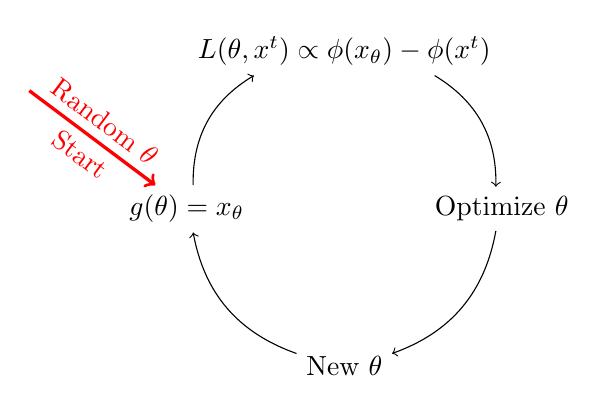
\begin{tikzpicture}[node distance=2cm, auto]

% Nodes
\node (start) [text centered] {\( g(\theta) = x_{\theta} \)};
\node (L) [above of=start, right of=start, text centered] 
    {\( L(\theta, x^t) \propto \phi(x_{\theta}) - \phi(x^t) \)};
\node (optimize) [below of=L, right of=L, text centered] {Optimize $\theta$};
\node (new_theta) [below of=optimize, right of=start, text centered] {New \( \theta \)};

% Highlight and arrow for the start node
\draw[->, very thick, red] (start) ++(-2,1.5) -- (start)
    node[midway, below, align=center, sloped, color=red] {Start}
    node[midway, above, align=center, sloped, color=red] {Random $\theta$};

% Arrows with multi-line labels
\draw[->, bend left] (start) to node[midway, right, align=center] {} (L);
\draw[->, bend left] (L) to node[midway, right, align=center] {} (optimize);
\draw[->, bend left] (optimize) to node[midway, below, align=center] {} (new_theta);
\draw[->, bend left] (new_theta) to node[midway, left, align=center] {} (start);

\end{tikzpicture}

    \caption{ Iterative approach to sound design. Adapted to OOD scenarios~\cite{salimi2025evaluating}.}
    \label{fig:sound_design_loop_iterative}
\end{figure}
\subsection{Problem Setup}

The methodology evaluates loss functions across multiple out-of-domain (OOD) sound-matching scenarios. Each experiment follows the iterative optimization loop in Fig.~\ref{fig:sound_design_loop_iterative}, where a synthesizer $g$ is optimized to imitate a target sound generated by a different synthesizer $g^{t}$. This iterative loop is the adaption of previous work by Salimi \textit{et. al.}~\cite{salimi2025evaluating}.

An \textit{experiment} consists of a complete optimization run: random parameter initialization, 200 steps of gradient-based optimization, and final parameter evaluation. Each experiment is defined by the following components, adapted to OOD settings from previous in-domain work~\cite{salimi2025evaluating,vahidi2023mesostructures}.

\begin{itemize}
    \item $g(\theta)$: A parametric audio synthesizer with parameters $\theta$ producing output $x_{\theta} = g(\theta)$.
    \item $g^{t}(\theta^{t})$: The target synthesizer producing the target sound $x^{t} = g^{t}(\theta^{t})$. OOD conditions require that $g$ and $g^{t}$ differ in structure or parameter ranges such that their output sets do not overlap.
    \item $x_{\theta}$: The imitator’s synthesized audio for parameters $\theta$.
    \item $x^{t}$: The target audio to be imitated.
    \item $\phi(\cdot)$: A feature representation function mapping waveforms into a comparison space.
    \item $L$: A loss function defined as $L(\theta, x^{t}) = d(\phi(x_{\theta}), \phi(x^{t}))$ for some metric $d$.
\end{itemize}

A \textit{scenario} is a group of four experiments---one for each of the four loss functions---performed with the same pair of synthesizers $(g, g^{t})$. Each scenario models a distinct sound-design task, such as matching filter cutoffs, modulation structure, or pitch trajectories, allowing us to evaluate how each loss function behaves under specific forms of OOD mismatch.

\subsection{Loss Functions}
\label{subsec:loss_functions}

We evaluate the same four loss functions used in the previous in-domain study~\cite{salimi2025evaluating}. The functions are summarized below:

\medskip
\noindent\textbf{\LoneSpec:}
This loss computes a pointwise L1 distance between the log-magnitude spectrograms of the imitator and target:
\begin{equation}
    L_{\mathrm{L1}}(\theta, x^{t}) 
    = \left\| STFT (x_{\theta}) - STFT (x^{t}) \right\|_{1}
\end{equation}

The STFT function uses 512 FFT bins, window size of 600 samples, and hop length of 100 samples~\cite{salimi2025evaluating}.

\medskip
\noindent\textbf{\SIMSESpec:}
The scale-invariant mean-squared error (SIMSE). This loss is identical to \LoneSpec, with the exception that it utilizes the SIMSE difference instead of L1.
\begin{equation}
    L_{\mathrm{SIMSE}}(\theta, x^{t}) 
    =  SIMSE( STFT (x_{\theta}) - STFT (x^{t}))
\end{equation}

\medskip
\noindent\textbf{\JTFS:}
The joint time-frequency scattering (JTFS) transform provides a multiresolution representation of temporal and spectral structures of time-series~\cite{vahidi2023mesostructures,anden2015joint}. The loss is defined as:
\begin{equation}
    L_{\mathrm{JTFS}}(\theta, x^{t})
    = 
    \left\|
        \Phi_{\mathrm{JTFS}}(x_{\theta})
        -
        \Phi_{\mathrm{JTFS}}(x^{t})
    \right\|_{2}
\end{equation}
Where $\phi$ is the application of L2 distance metric to the 1-Dimensional JTFS transform provided by Andreux \textit{et. al}~\cite{kymatio,salimi2025evaluating}.

\medskip
\noindent\textbf{\DTWEnv:}
This loss computes a dynamic time-warping (DTW) distance between amplitude envelopes. Since the original DTW function is not differentiable, the soft-DTW distance is used instead~\cite{softdtw_jax}. The envelope of the sound is calculated by taking the STFT, and summing the values of all frequency bins at every time-step~\cite{salimi2025evaluating}.

\begin{equation}
    L_{\mathrm{DTW}}(\theta, x^{t})
    =
    \mathrm{DTW}
    \left(
        \mathrm{Env}(x_{\theta}),
        \mathrm{Env}(x^{t})
    \right).
\end{equation}

\subsection{Evaluation Methods}
\label{subsec:evaluation}
 Evaluations are the scores associated with every experiment, which are later used to determine which loss function is the best performer for which scenario. 

 We have two evaluation methods: human similarity ratings (or likert scores) from a small listening survey, and the automatic partial P-Loss (PPL), which we introduce in this paper as a reasonable measure of performance in OOD settings. 

\subsubsection{Partial P-Loss}
\label{sec:partial_ploss}
In out-of-domain sound-matching, many parameters of the target and imitator synthesizers do not correspond directly; for example, when the target employs a saw oscillator but the imitator uses noise, or when modulation structures differ.  
To evaluate only the aspects of the signal that can meaningfully transfer across domains, we compute a \emph{partial parameter loss} (PPL).  

PPL measures the L2 distance only across the subset of parameters considered perceptually critical for the scenario:
\begin{equation}
\mathrm{PPL} = \| \theta^{(\mathrm{crit})}_t - \hat{\theta}^{(\mathrm{crit})} \|_2,
\end{equation}
where $\theta^{(\mathrm{crit})}$ denotes the target’s critical parameters (e.g., filter cutoffs, modulation rates) and $\hat{\theta}^{(\mathrm{crit})}$ the corresponding recovered parameters of the imitator.  
Parameters with no perceptual or structural correspondence are ignored. 
If done correctly, this can enable a reasonable interpretable comparison across mismatched synthesizers. The PPL for each scenario will be unique, and we will highlight which parameters are used as we describe the scenarios later on.

\subsubsection{Hearing tests}
Hearing tests are the gold standard for measuring performance of sound-matching algorithms. For each scenario, we randomly sample 40 sound-pairs for each loss, and two of the authors listen to the 160 samples in a blinded manner (not knowing which loss was used in the iterative loop). The authors give a Likert score of 1 (not similar at all) to 5 (near identical) to these sound-pairs. These scores are then combined for a total of 320 manual given performance measures for each scenario. 

\subsection{Optimization Loop}
\label{subsec:optimization}


\todo{This contradicts something you've said previous about experiments so decide if you want to keep the definition of experiments the same as before or change it and add trial}A \textit{trial} is defined as one complete 200-step optimization run with a single target sample. An \textit{experiment} consists of 300 independent trials using the same target synthesizer $g^{t}$, imitator synthesizer $g$, and loss function $L$. A \textit{scenario} consists of four experiments that share the same synthesizer pair $(g, g^{t})$ but use different loss functions.

Each trial consists of a 200-iteration gradient-based optimization procedure. Starting from a random initialization $\theta_{0}$, following past work, the imitator synthesizer parameters are updated using the RMSProp optimizer with a fixed learning rate of 0.045~\cite{salimi2025evaluating}.

All synthesizers are implemented in Faust and transpiled into differentiable JAX functions using DawDreamer~\cite{braun2024dac}. 

\subsection{Boostrapping and Ranking Procedures}
\label{subsec:ranking}

We perform all statistical comparisons using bootstrapped performance distributions. For each experiment, the 300 trial-level scores for PPL or 80 scores from survey results are resampled with replacement, and 1000 bootstrapped means are computed. These 1000 values form an empirical distribution that avoids parametric assumptions about the underlying score distribution, and simplifies comparisons between the two performance measures~\cite{chernick2011bootstrap}.

To compare loss functions within a scenario, we apply the nonparametric Scott--Knott procedure (NPSK). For each performance measure, NPSK recursively partitions the bootstrapped distribution to maximize between-group separation while minimizing within-group variance, producing statistically justified ranks without requiring normality~\cite{tantithamthavorn2017mvt,tantithamthavorn2018optimization}. Rank~1 corresponds to the best-performing distribution, with larger ranks indicating worse performance. Ties occur when two or more distributions cannot be statistically distinguished under the NPSK splitting criterion, resulting in equal assigned ranks.

\section{Scenarios and Results}
\todo{What are you going to describe? and mention sampling rate is set to 48000}
\subsection{Band Pass Matching}
In this scenario, the two synthesizers are the application of band-passing to noise (\BPNoise) and saw waves (\BPSaw). Examples of these programs are given in Listings~\ref{lst:program0} and ~\ref{lst:program0_saw} respectively. Previous observations have shown that with in-domain sound-matching of \BPNoise, the loss functions utilizing spectrogram differences were the best performers, speculating that this due to the clear visibility of filter-cutoffs in a spectrogram~\cite{salimi2025evaluating}. 
 
 Here we use \BPSaw as the target synthesizer, and \BPNoise as the imitator. We define success in sound-matching here as the L2 distance of the imitator's high and low-pass cutoffs to the corresponding parameters in the target synthesizer. This creates an out-of-domain experiment where PP-Loss is an objective measure of success. 

Like previous work, hearing tests reveal the spectrogram based losses as appropriate for band-passing~\cite{salimi2025evaluating}. As shown in Table~\ref{tab:scenario_ranks}, both hearing tests and PP-Loss determine \SIMSESpec to be the best performing loss function for the band-passing scenario. However, there are differences in how ranks 2-4 were assigned. 
 
\begin{table*}[t]
\centering
\small
\setlength{\tabcolsep}{4pt}
\renewcommand{\arraystretch}{1.15}
\resizebox{\textwidth}{!}{%
\begin{tabular}{|l|cc|cc|cc|cc|cc|cc|cc|}
\hline
\textbf{Loss} 
& \multicolumn{2}{|c|}{\textbf{AM: non-overlap}} 
& \multicolumn{2}{c|}{\textbf{AM: sine $\rightarrow$ saw}} 
& \multicolumn{2}{c|}{\textbf{AM: saw $\rightarrow$ sine}} 
& \multicolumn{2}{c|}{\textbf{BP: noise $\rightarrow$ saw}} 
& \multicolumn{2}{c|}{\textbf{Chirp: delayed}} 
& \multicolumn{2}{c|}{\textbf{Chirp: pulsating}} 
& \multicolumn{2}{c|}{\textbf{Chirp: no delay}} \\
\cline{2-15}
& \textbf{PP-Loss} & \textbf{Hearing}
& \textbf{PP-Loss} & \textbf{Hearing}
& \textbf{PP-Loss} & \textbf{Hearing}
& \textbf{PP-Loss} & \textbf{Hearing}
& \textbf{PP-Loss} & \textbf{Hearing}
& \textbf{PP-Loss} & \textbf{Hearing}
& \textbf{PP-Loss} & \textbf{Hearing} \\
\hline
SIMSE & 2 & 3 & 3 & 1 & 2 & 2 & 1 & 1 & 3 & 3 & 2 & 2 & 3 & 3 \\
L1    & 3 & 2 & 4 & 2 & 4 & 1 & 3 & 2 & 4 & 4 & 3 & 3 & 2 & 1 \\
JTFS  & 4 & 4 & 2 & 3 & 3 & 2 & 4 & 4 & 1 & 1 & 2 & 2 & 1 & 1 \\
DTW   & 1 & 1 & 1 & 3 & 1 & 3 & 2 & 3 & 2 & 2 & 1 & 1 & 4 & 4 \\
\hline
\end{tabular}%
}
\caption{Summary of ranks across seven scenarios using two evaluation measures: bootstrapped PP-Loss and bootstrapped hearing survey ratings. Lower rank indicates better performance.}
\label{tab:scenario_ranks}
\end{table*}


\begin{figure*}[htbp]
  \centering
  \scriptsize

  %-------------------------------------%
  % Left panel
  %-------------------------------------%
  \begin{minipage}{0.48\textwidth}
    \begin{minipage}{0.10\textwidth}
      \raggedleft
      \vspace{0.5cm}
      SIMSE\\[0.6cm]
      L1\\[0.65cm]
      JTFS\\[0.65cm]
      DTW
    \end{minipage}%
    \begin{minipage}{0.87\textwidth}
      \centering
      \includegraphics[width=\linewidth]{images/npsk_ood_P_Loss_3.png}
    \end{minipage}
  \end{minipage}
  \hfill
  %-------------------------------------%
  % Right panel
  %-------------------------------------%
  \begin{minipage}{0.48\textwidth}

    \begin{minipage}{0.87\textwidth}
      \centering
      \includegraphics[width=\linewidth]{images/npsk_ood_likert_3.png}
    \end{minipage}
  \end{minipage}

  \caption{Bootstrapped distributions and NPSK ranks for two band-pass matching setups.}
  \label{fig:npsk_BP_two}
\end{figure*}



\begin{lstlisting}[caption={\BPNoise}, label={lst:program0}, language=Faust,
                  float, floatplacement=!H, xleftmargin=1em, xrightmargin=0.5em, firstnumber=0, aboveskip=0em, belowskip=-1em]
import("stdfaust.lib");
lp_cut = hslider("lp_cut",900,100,5000,5);
hp_cut = hslider("hp_cut",100,1,400,5);
process = no.noise:fi.lowpass(3,lp_cut):fi.highpass(10,hp_cut);
\end{lstlisting}

\begin{lstlisting}[caption={\BPSaw}, label={lst:program0_saw}, language=Faust,
                  float, floatplacement=!H, xleftmargin=1em, xrightmargin=0.5em, firstnumber=0, aboveskip=0em, belowskip=-1em]
import("stdfaust.lib");
lp_cut = hslider("lp_cut", 2801, 100, 5000, 1);
hp_cut = hslider("hp_cut", 142, 1, 400, 1);
sawOsc(f) = +(f/ma.SR) ~ ma.frac;
process = sawOsc(30):fi.lowpass(5, lp_cut):fi.highpass(5, hp_cut);
\end{lstlisting}



\subsection{AM-Synthesizer Matching}
\begin{lstlisting}[caption={\FMMod}, label={lst:program3},language=Faust,float,floatplacement=!H,xleftmargin=1em,xrightmargin=0.5em,firstnumber=0,aboveskip=0em, belowskip=-1em]
import("stdfaust.lib");
carrier = hslider("car",car_a,car_b,car_c,1);
amp = hslider("amp",amp_a,amp_b,amp_c,1);
sineOsc(f) = +(f/ma.SR) ~ ma.frac:*(2*ma.PI) : sin;
sawOsc(f) = +(f/ma.SR) ~ ma.frac;
process = sineOsc(amp)*sawOsc(car);
\end{lstlisting}


\begin{lstlisting}[caption={\FMModvtwo}, label={lst:program3_v2},language=Faust,float,floatplacement=!H,xleftmargin=1em,xrightmargin=0.5em,firstnumber=0,aboveskip=0em, belowskip=-1em]
import("stdfaust.lib");
carrier = hslider("car",car_a,car_b,car_c,1);
amp = hslider("amp",amp_a,amp_b,amp_c,1);
sineOsc(f) = +(f/ma.SR) ~ ma.frac:*(2*ma.PI) : sin;
process = sineOsc(amp)*sineOsc(car);
\end{lstlisting}


\label{sec:am_sound_matching}
We test three OOD scenarios for AM-Synthesizers. \FMMod and \FMModvtwo as described in Listings~\ref{lst:program3} and~\ref{lst:program3_v2} are the basis for the three variations of this scenario. \FMMod generates a sound by modifying the amplitude of a saw oscillator with a sinusoidal LFO. \FMModvtwo is a modification which uses sine oscillators for both the carrier and the modulator. In this section, we will refer to the LFO frequency as \texttt{amp} and carrier frequency as \texttt{car}. The value of \texttt{amp} shapes the amplitude of the sound (or the wobbling effect), and \texttt{car} determines the frequency of the sound.

In these scenarios, the \texttt{amp} values can match, but the frequency content cannot. In version 1 (Non-Overlapping Frequencies), the range of available frequencies are different. In version 2 (Sine Target, Saw Imitator), the imitator can only make sine tones while the target can only makes saw waves, and vice versa for scenario 3 (Saw Target, Sine Imitator). A question we have to consider is: how would we match the sounds manually? Here we see why OOD experiments are difficult, as describing sound similarity can be quite subjective.

If the carrier frequencies could not possibly match (as in scenario 1), the best method for matching the carrier frequencies is not clear. Although the distances between the frequencies can be reduced, there will always be a gap. What's more, matching musical notes is not simply a matter of frequency values. For example, let's consider the commonly used equal temperament tuning system~\cite{sethares2005tuning}, where the A4 note is usually associated with 440 Hz. In this system, if the target synth is producing a frequency at 440 Hz, and the imitator can only produce values below 400 Hz, then the correct objective for the frequency is dependent on the sound designers needs. 400Hz might be the best frequency parameter, since it is as close as we can get to 440Hz; or perhaps the value of 220 Hz (corresponding to A3) is a better match than the value of 392 Hz (corresponding to G4). In general, considering the commonly used logarithmic scaling of musical notes, it can be argued that the best matches for any frequency $f$ are $f*2^{n}$, where n is any integer~\cite{young1939terminology}. \todo{(does this tie back into the hypothesis that the sinusoidal nature of sound can cause non-smooth loss functions)}

We ignore the frequency parameter for the PPL definition, and take the proximity of \texttt{amp} values as a reasonable measure of success: not only can the \texttt{amp} values between the imitator and target have the same range, but also the transfer of the amplitude changes from one sample to another is a common sound-design task \cite{engel2020ddsp}. To measure sound matching success, the PPL is set to the squared difference between the amp values in $\theta_t$ and the output parameters.

\subsubsection{Non-Overlapping frequencies}
\label{sec:am_sound_matching_nonoverlapping}
For this scenario, we choose two instances of \FMModvtwo, with the carriers having non-overlapping frequency ranges of 30-250 Hz for the target synth and 1000-5000 Hz for the imitator. Here, the carrier is a sine oscillator, therefore the clashing of higher harmonics can be factored out as a source of confusion in the loss function landscape. Since there is no overlap in the carrier frequency ranges, the tone of the imitator and target synth can never match, making this a simple out-of-domain scenario. As shown in Table~\ref{tab:scenario_ranks}, \DTWEnv outperforms other loss functions in both PPL and hearing tests, and \JTFS is the worst performer.

\subsubsection{Sine Target, Saw Imitator}
\label{sec:am_sinetarget_sawimitate}
In this scenario, we select \FMModvtwo as the target, and \FMMod as the imitator, both with \texttt{amp} ranges of 1-15 Hz and \texttt{car} range of 30-5000 Hz. Here we again see that the \DTWEnv function objectively finds the closest amplitude value, yet the hearing tests align with the spectrogram based losses. A likely explanation here is that \DTWEnv clearly excels at finding the correct amp parameter, it ignores frequency content, which leads to low rankings assigned by manual listeners. 


\subsubsection{Saw Target, Sine Imitator}
\label{sec:am_sawtarget_sineimitate}
This scenario uses \FMMod as the target and \FMModvtwo as the imitator, we also see here that \DTWEnv is the best performer according to PPL, but manual raters are partial to the spectrogram based losses,  likely due to reasons discussed in the previous sub-scenario.

\begin{figure}[t]
  \centering
  \begin{minipage}[t]{\textwidth}
    % Left-side labels
    \begin{minipage}[t]{0.045\textwidth}
      \footnotesize\raggedleft
      \vspace{-2.75cm} % align with top of images
      SIMSE\\[0.4cm]
      L1\\[0.385cm]
      JTFS\\[0.365cm]
      DTW
    \end{minipage}%
    \hspace{0.01\textwidth}%
    % Right side: images + captions
    \begin{minipage}[t]{0.91\textwidth}
      \centering
      \begin{minipage}[t]{0.31\textwidth}
        \centering
        \includegraphics[width=\linewidth]{images/npsk_ood_P_Loss_0.png}
        \vspace{0.3em}
        \footnotesize Non-Overlapping Frequencies
      \end{minipage}
      \hspace{0.015\textwidth}%
      \begin{minipage}[t]{0.31\textwidth}
        \centering
        \includegraphics[width=\linewidth]{images/npsk_ood_P_Loss_1.png}
        \vspace{0.3em}
        \footnotesize Sine Target, Saw Imitator
      \end{minipage}
      \hspace{0.01\textwidth}%
      \begin{minipage}[t]{0.31\textwidth}
        \centering
        \includegraphics[width=\linewidth]{images/npsk_ood_P_Loss_2.png}
        \vspace{0.3em}
        \footnotesize Saw Target, Sine Imitator
      \end{minipage}
    \end{minipage}
  \end{minipage}
  \caption{Bootstrapped distributions and ranks for AM-Synthesizer sound matching.}
  \label{fig:npsk_am_synths}
\end{figure}
\begin{figure*}[t]
  \centering
  % Left-side labels
  \begin{minipage}[t]{0.045\textwidth}
    \footnotesize\raggedleft
    \vspace{-3cm} % align with top of images
    SIMSE\\[0.4cm]
    L1\\[0.385cm]
    JTFS\\[0.365cm]
    DTW
  \end{minipage}%
  \hspace{0.01\textwidth}%
  % Right-side: reordered minipage images
  \begin{minipage}[t]{0.94\textwidth}
    \centering
    \begin{minipage}[t]{0.31\textwidth}
      \centering
      \includegraphics[width=\linewidth]{images/npsk_ood_P_Loss_6.png}
      \vspace{0.3em}
      \footnotesize (a)~Delayed Pitch-bend
    \end{minipage}
    \hspace{0.015\textwidth}
    \begin{minipage}[t]{0.31\textwidth}
      \centering
      \includegraphics[width=\linewidth]{images/npsk_ood_P_Loss_4.png}
      \vspace{0.3em}
      \footnotesize (b)~No-delay Pitch-bend
    \end{minipage}
    \hspace{0.015\textwidth}
    \begin{minipage}[t]{0.31\textwidth}
      \centering
      \includegraphics[width=\linewidth]{images/npsk_ood_P_Loss_5.png}
      \vspace{0.3em}
      \footnotesize (c)~Pulsating Pitch-bend
    \end{minipage}
  \end{minipage}
  \caption{Bootstrapped distributions and ranks for non-delayed, randomly delayed, and pulsating pitch-bend programs.}
  \label{fig:npsk_pitch_bends}
\end{figure*}

\subsection{Pitch-Bending}
Vahidi et al. showed that \JTFS out-performs MSS in in-domain sound-matching of chirplet synthesizers~\cite{vahidi2023mesostructures}. Chirplets are tones which increase in frequency at an exponential rate, the frequency of the tone and the rate of increase being the two major parameters. Here we test three different scenarios with pitch-bending synthesizers that resemble chirplets. The main scenario (Delayed Pitch-Bending) is OOD, where the chirplets have a randomly assigned built-in delay offset. The second scenario is in-domain, where we eliminate the random delay to see the effect on performance. We introduce a third scenario (pulsating Pitch-bend) that is also in-domain, but the chirplet frequency does not strictly increase linearly on a log-scale. 


\subsubsection{Delayed Pitch-Bending}
The program here is a sine wave with a steady starting pitch for a random amount of time; after a time delay of 5000-30000 samples, an exponential upward pitch bend is applied to the starting pitch. The search parameters here are the starting pitch (30-500 Hz) and the rate at which the power of the exponent increases (1-20 samples at every time step). The time-delay for the pitch-bending onset is selected randomly for each experiment, so it is very unlikely that the imitator would be able to replicate the target's sounds, making this an out-of-domain example.

This scenario shows identical ratings between both PPL and hearing tests. Both measures show \JTFS as the best performing loss, which is consistent with the findings of Vahidi et al. which showed \JTFS to be agnostic to slight perturbations in the frequency and time scale, at least when matching chirplet synthesizers\cite{vahidi2023mesostructures}.

\subsubsection{No-Delay Pitch-Bending}
As a follow-up experiment, we conducted the \textit{in-domain} comparison of pitch-bending synthesizers \textit{without} delay. This scenario would be a close replication of the original in-domain experiments by Vahidi \textit{et. al.}. In other words, it is identical to the delayed pitch-bending experiment but the delay variable $\delta$ is always set to 0 (see Listing~\ref{lst:pitchbendup}). As expected, \JTFS remains the best performer according to PPL and hearing tests.

\subsubsection{Pulsating Pitch-Bending}
Vahidi et al. contended that \JTFS is the appropriate loss function for the capture of ``mesostructures''. Previous work has shown that this is not always the case with in-domain scenarios~\cite{salimi2025evaluating}. As shown in Listing~\ref{lst:pitchbendup_pulse}, this scenario adds a pulse to the pitch-bending synthesizer, such that the frequency is shifted upwards overall, but also pulsing up and down within a narrow range. This characteristic is fully within the definition of ``mesostructure'', yet \JTFS is outperfomed by \DTWEnv according to PPL and hearing tests. 

% Another conclusion here is that all loss function perform much worse on the proximity scale

Here, we can define success with P-Loss, that is, how well the \texttt{increase\_speed} and \texttt{starting\_pitch} parameters are approximated despite the delay in the pitch-bending onset. Figure~\ref{fig:npsk_pitch_bends} the right side shows that \JTFS is the best performing loss function, which is consistent with the previous findings by Vahidi \textit{et al.}~\cite{vahidi2023mesostructures}. 



\begin{lstlisting}[escapeinside={(*}{*)},caption={\PitchBendUp program. when an instance of the synthezier is created, $\delta$ is randomly assigned a value between 5000-30000 samples (Delayed Pitch-bend) or set to 0 (No-delay Pitch-bend)}, label={lst:pitchbendup},language=Faust,float,floatplacement=!H,xleftmargin=1em,xrightmargin=0.5em,firstnumber=0,aboveskip=0em, belowskip=-1em]
import("stdfaust.lib");
increase_speed = hslider("increase_speed",2,1,20,0.1);
starting_pitch = hslider("starting_pitch",200,30,500,0.1);
sineOsc(f) = +(f/ma.SR) ~ ma.frac:*(3*ma.PI):sin;
increasing_pitch(rate) = _ ~+(rate/ma.SR):exp;
process = sineOsc(increasing_pitch(increase_speed):de.delay((*$\delta$*),48000)+starting_pitch);

\end{lstlisting}

\begin{lstlisting}[escapeinside={(*}{*)},caption={\textbf{Pulsating PitchBend}}, label={lst:pitchbendup_pulse},language=Faust,float,floatplacement=!H,xleftmargin=1em,xrightmargin=0.5em,firstnumber=0,aboveskip=0em, belowskip=-1em]
import("stdfaust.lib");
increase_speed = hslider("increase_speed", 4.57, 2, 7, 0.1);
pulse_rate = hslider("pulse_rate", 3.93, 1, 10, 0.1);
sineOsc(f) = +(f/ma.SR) ~ ma.frac : *(3*ma.PI) : sin;
sawOsc(f) = +(f/ma.SR) ~ ma.frac : +(0.5);
increasing_pitch(rate) = _ ~ +(rate/ma.SR) : exp;
process = sineOsc(30 + increasing_pitch(increase_speed) + sawOsc(pulse_rate) * 526);
\end{lstlisting}
% \section{Gradients}
% Different forms of gradient analysis has been conducted in previous works~\cite{masuda2023improving,turian2020sorry,vahidi2023mesostructures}.


\section{Discussion}
\subsection{Key Findings}
In the BP scenario, we see that \SIMSESpec is the best performer, which is consistent with previous findings, and highlights \SIMSESpec as an alternative to the commonly used application of L1 and L2 distances to spectrograms~\cite{turian2020sorry}.

AM-Synthesis results are chaotic. In the non-overlapping frequencies scenario, \DTWEnv is the best performer due to its sole focus on changes in sound-envelope. However, when harmonics imperfectively overlap in the sine-to-saw and saw-to-sine scenarios, \DTWEnv outperforms other losses in finding the closest amplitude modulation frequency, but hearing tests show a prefernce for spectrogram based losses. This further solidifies the utility of DTW bases losses in sound-design, but highlights its limitation in harmonic adjustments. 

The three chirplet scenarios show perfect matching between both PP-Loss and hearing tests. In the delayed and no-delay matching scenarios which resemble previous work by Vahidi \textit{et al.} confirm the utility of \JTFS in chirplet matching. However, we see that a slight variation on this setup as shown by the pulsating chirplet scenario favors \DTWEnv. This further questions the suitability of \JTFS as a loss function for ``mesostructures'' as a whole~\cite{vahidi2023mesostructures}.

In 5 out of the 7 scenarios, the PP-Loss and Hearing tests had identical first rank ratings. This shows that a well designed and justified PP-Loss could be utilized in automated OOD experiments. 




\section{Conclusion}
\clearpage
\bibliographystyle{alpha}

\bibliography{references}


\end{document}
